% Monografia-LaTeX (Unochapecó)                                           %
% Copyright (C) 2013  Daniel Girotto                                      %
%                                                                         %
% This program is free software: you can redistribute it and/or modify    %
% it under the terms of the GNU General Public License as published by    %
% the Free Software Foundation, either version 3 of the License, or       %
% (at your option) any later version.                                     %
%                                                                         %
% This program is distributed in the hope that it will be useful,         %
% but WITHOUT ANY WARRANTY; without even the implied warranty of          %
% MERCHANTABILITY or FITNESS FOR A PARTICULAR PURPOSE.  See the           %
% GNU General Public License for more details.                            %
%                                                                         %
% You should have received a copy of the GNU General Public License       %
% along with this program.  If not, see <http://www.gnu.org/licenses/>.   %

% ------------------------------------------------------------ %
% Monografia                                                   %
% ------------------------------------------------------------ %
\documentclass[pnumromarab, normaltoc, a4paper, 12pt]{abnt-unochapeco}

\usepackage{url}
\usepackage{leading}
\usepackage{lmodern}
\usepackage{graphicx}
\usepackage[abnt-emphasize=bf]{abnt-alf}
\usepackage{varwidth}
\usepackage[T1]{fontenc}
\usepackage[latin1]{inputenc}
\usepackage[brazil]{babel}

\begin{document}

\newcommand{\area}{área de ciências exatas e ambientais}
\newcommand{\curso}{ciência da computação}
\newcommand{\grau}{bacharelado}
\newcommand{\grautitulo}{bacharel}
\newcommand{\supervisortcc}{Prof. Fulano da Silva, Esp.,MSc., Dr.}
\newcommand{\coordenador}{Prof. Outro Fulano, Esp.,MSc., Dr.}
\newcommand{\membrobancaa}{Prof. Fulano da Silva, Esp.,MSc., Dr.}
\newcommand{\membrobancab}{Prof. Outro Fulano, Esp.,MSc., Dr.}
\newcommand{\datadefesa}{Dia de Mês de Ano (data da defesa)}

\renewcommand{\autor}{nome completo do aluno}
\renewcommand{\instituicao}{universidade comunitária da região de chapecó}
\renewcommand{\titulo}{título do trabalho de conclusão do curso}
\renewcommand{\local}{Chapecó}
\renewcommand{\data}{mês (extenso) de ano (4 dígitos)}
\renewcommand{\comentario}{Relatório do Trabalho de Conclusão de Curso submetido
  à Universidade \mbox{Comunitária} da Região de Chapecó para obtenção do título
  de bacharelado no curso de Ciência da Computação.}
\renewcommand{\orientador}{Prof(a). Nome do(a) orientador(a)}
\renewcommand{\coorientador}{Prof(a). Nome do(a) co-orientador(a)}

\capa
\folhaderosto
\folhadeaprovacao

% Monografia-LaTeX (Unochapec�)                                           %
% Copyright (C) 2013  Daniel Girotto                                      %
%                                                                         %
% This program is free software: you can redistribute it and/or modify    %
% it under the terms of the GNU General Public License as published by    %
% the Free Software Foundation, either version 3 of the License, or       %
% (at your option) any later version.                                     %
%                                                                         %
% This program is distributed in the hope that it will be useful,         %
% but WITHOUT ANY WARRANTY; without even the implied warranty of          %
% MERCHANTABILITY or FITNESS FOR A PARTICULAR PURPOSE.  See the           %
% GNU General Public License for more details.                            %
%                                                                         %
% You should have received a copy of the GNU General Public License       %
% along with this program.  If not, see <http://www.gnu.org/licenses/>.   %

% ------------------------------------------------------------ %
% Dedicat�ria
% ------------------------------------------------------------ %
\vspace*{20cm}
\hspace{0.4\textwidth}
\begin{varwidth}{0.48\textwidth}
  \leading{5mm}
  Dedico.....\\
  Item OPCIONAL, deve ficar posicionado ao final da folha.\\
  � uma men��o onde o autor presta \mbox{homenagem} ou dedica o trabalho a
  algu�m
\end{varwidth}
% Monografia-LaTeX (Unochapec�)                                           %
% Copyright (C) 2013  Daniel Girotto                                      %
%                                                                         %
% This program is free software: you can redistribute it and/or modify    %
% it under the terms of the GNU General Public License as published by    %
% the Free Software Foundation, either version 3 of the License, or       %
% (at your option) any later version.                                     %
%                                                                         %
% This program is distributed in the hope that it will be useful,         %
% but WITHOUT ANY WARRANTY; without even the implied warranty of          %
% MERCHANTABILITY or FITNESS FOR A PARTICULAR PURPOSE.  See the           %
% GNU General Public License for more details.                            %
%                                                                         %
% You should have received a copy of the GNU General Public License       %
% along with this program.  If not, see <http://www.gnu.org/licenses/>.   %

% ------------------------------------------------------------ %
% Agradecimento
% ------------------------------------------------------------ %
\vspace*{18.5cm}
\hspace{0.4\textwidth}
\begin{varwidth}{0.48\textwidth}
  \leading{5mm}
  Agrade�o....\\
  Item OPCIONAL, deve ficar posicionado ao final da folha.\\
  S�o men��es a pessoas e/ou institui��es das quais eventualmente recebeu apoio
  e que concorreram de maneira relevante para o desenvolvimento do trabalho.
\end{varwidth}
% Monografia-LaTeX (Unochapec�)                                           %
% Copyright (C) 2013  Daniel Girotto                                      %
%                                                                         %
% This program is free software: you can redistribute it and/or modify    %
% it under the terms of the GNU General Public License as published by    %
% the Free Software Foundation, either version 3 of the License, or       %
% (at your option) any later version.                                     %
%                                                                         %
% This program is distributed in the hope that it will be useful,         %
% but WITHOUT ANY WARRANTY; without even the implied warranty of          %
% MERCHANTABILITY or FITNESS FOR A PARTICULAR PURPOSE.  See the           %
% GNU General Public License for more details.                            %
%                                                                         %
% You should have received a copy of the GNU General Public License       %
% along with this program.  If not, see <http://www.gnu.org/licenses/>.   %

% ------------------------------------------------------------ %
% Ep�grafe
% ------------------------------------------------------------ %
\vspace*{18.5cm}
\hspace{0.4\textwidth}
\begin{varwidth}{0.5\textwidth}
  \leading{5mm}
  \raggedleft
  Ep�grafe\\
  Item OPCIONAL, deve ficar posicionado ao final da folha.\\
  � a inscri��o de um trecho em prosa ou composi��o po�tica que de certa forma
  embasou a constru��o do trabalho, seguida da indica��o de autoria.\\
  Fulano de tal
\end{varwidth}
% Monografia-LaTeX (Unochapec�)                                           %
% Copyright (C) 2013  Daniel Girotto                                      %
%                                                                         %
% This program is free software: you can redistribute it and/or modify    %
% it under the terms of the GNU General Public License as published by    %
% the Free Software Foundation, either version 3 of the License, or       %
% (at your option) any later version.                                     %
%                                                                         %
% This program is distributed in the hope that it will be useful,         %
% but WITHOUT ANY WARRANTY; without even the implied warranty of          %
% MERCHANTABILITY or FITNESS FOR A PARTICULAR PURPOSE.  See the           %
% GNU General Public License for more details.                            %
%                                                                         %
% You should have received a copy of the GNU General Public License       %
% along with this program.  If not, see <http://www.gnu.org/licenses/>.   %

% ------------------------------------------------------------ %
% Resumo
% ------------------------------------------------------------ %
\thispagestyle{empty}
\begin{center}
  \vspace*{.85cm}
  \textbf{RESUMO}
\end{center}

\vspace{2.5cm}
\noindent
\leading{5.5mm}
� a apresenta��o concisa do texto, destacando seus aspectos de maior relev�ncia.
� redigido em um �nico par�grafo, contendo entre 250 e 500 palavras. Usar
terceira pessoa do singular. N�o usar cita��es bibliogr�ficas. Ressaltar
objetivos, m�todos, resultados e conclus�es do trabalho.

\vspace{1.3cm}

\noindent
\textbf{Palavras-chave:} entre tr�s e cinco palavras-chave, separadas por ponto
e v�rgula.
% Monografia-LaTeX (Unochapec�)                                           %
% Copyright (C) 2013  Daniel Girotto                                      %
%                                                                         %
% This program is free software: you can redistribute it and/or modify    %
% it under the terms of the GNU General Public License as published by    %
% the Free Software Foundation, either version 3 of the License, or       %
% (at your option) any later version.                                     %
%                                                                         %
% This program is distributed in the hope that it will be useful,         %
% but WITHOUT ANY WARRANTY; without even the implied warranty of          %
% MERCHANTABILITY or FITNESS FOR A PARTICULAR PURPOSE.  See the           %
% GNU General Public License for more details.                            %
%                                                                         %
% You should have received a copy of the GNU General Public License       %
% along with this program.  If not, see <http://www.gnu.org/licenses/>.   %

% ------------------------------------------------------------ %
% Abstract
% ------------------------------------------------------------ %
\thispagestyle{empty}
\begin{center}
  \vspace*{.95cm}
  \textbf{ABSTRACT}
\end{center}

\vspace{2.5cm}
\noindent
\leading{5.5mm}
It is a brief presentation of the text in English, where the most relevant
aspects are underlined. It should be written in the third person singular, in an
only paragraph containing from 250 to 500 words. You should not mention
references. It is important to write the objectives, method, results and the
final remarks of the study.

\vspace{1.3cm}

\noindent
\textbf{Keywords:} from 3 to 5 keywords, separated by semicolon.

\addcontentsline{toc}{chapter}{LISTA DE SIGLAS}
\listadesiglas

\addcontentsline{toc}{chapter}{LISTA DE FIGURAS}
\listoffigures

\addcontentsline{toc}{chapter}{LISTA DE TABELAS}
\listoftables

% ------------------------------------------------------------ %
% Altera o título do Sumário                                   %
% ------------------------------------------------------------ %
\renewcommand{\contentsname}%
  {\vspace*{.8cm}
  \normalsize{\bfseries\MakeUppercase{sumário}}%
  \vspace{1.4cm}}

\sumario

\chapter{introdução}
\section{Contextualização}
No texto da apresentação, aborde o tema do trabalho iniciando por uma discussão
ampla do conteúdo, até tratar especificamente o que vai ser desenvolvido.
Fazendo uma analogia a uma pirâmide invertida, o texto poderia ficar assim
distribuído:

\begin{figure}[hbtp]
  \begin{center}
  \caption{Estrutura do item Apresentação(Item 1.1)}
  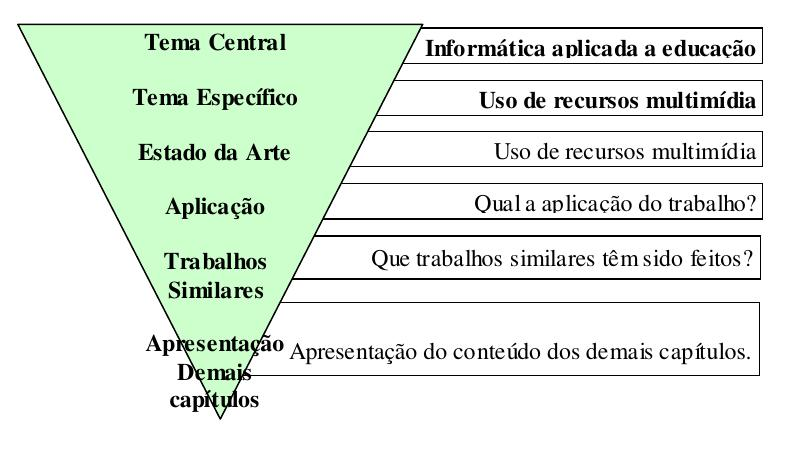
\includegraphics[width=150mm]{images/imagem1.jpeg}
  \end{center}
\end{figure}

\section{Delimitação do problema}
Aqui você coloca o problema a ser trabalhado no TCC. Analise se o que você está
colocando não é um objetivo. Lembre-se, ``implementar alguma coisa não é
problema, mas sim, objetivo''.

\section{Justificativa}
Aqui você vai dizer porquê trabalhar o problema acima é importante para a área
da computação ou para o futuro usuário.

Procure embasar a justificativa com citações de autores que você esteja
estudando.\\
\\

\section{Objetivos}
\subsection{Objetivo geral}
Geralmente é um único parágrafo que contém o grande objetivo de trabalhar o tema
escolhido, ou seja, o principal objetivo do TCC é ...

\subsection{Objetivos específicos}
A partir do objetivo geral, são detalhados alguns objetivos específicos que irão
delimitar mais ainda o tema abordado no TCC. Geralmente são colocados na forma
de itens. É um detalhamento do objetivo geral.

\begin{itemize}
  \leading{5mm}
  \item [] a) ...
  \item [] b) ...
  \item [] c) ...
\end{itemize}

\section{Procedimentos Metodológicos}
Primeiramente, caracterize o teu trabalho relacionado ao tipo de pesquisa quanto
aos objetivos.

Após, juntamente com o Orientador, você deve descrever detalhadamente como serão
desenvolvidos os trabalhos do TCC. Procure pensar que você está fazendo uma
receita de bolo e quem quiser fazer um TCC igual ao seu, ou validá-lo para ver
se está correto, deverá seguir detalhadamente esta receita.

Descreva como cada etapa será desenvolvida no decorrer do trabalho, enriquecendo
com detalhes específicos de cada etapa.

\section{Estrutura do Trabalho}
Apresentar a estrutura do trabalho, ou seja, como ele está estruturado em
termos de capítulos a partir da revisão bibliográfica.

\chapter{NORMAS PARA DIGITAÇÃO DO TRABALHO DE CONCLUSÃO DE CURSO}
O segundo capítulo visa apresentar conceitos e trabalhos relacionados ao tema.
Quanto a estrutura da revisão bibliográfica pode ser apresentada em um ou mais
capítulos, dependerá do tema abordado. Caso optar por fazer mais de um capítulo
de revisão, fica estabelecido no máximo 3 capítulos para revisão bibliográfica.
\begin{itemize}
  \leading{5mm}
  \item [] 2.1 - xxx
  \item [] 2.2 - yyy
\end{itemize}
No caso de capítulo único: a revisão bibliográfica deverá ser feita em
subcapítulos por temáticas. Ex.: 2.1 - O ramo atacadista no oeste de SC. 2.2
Tecnologias da Informação. Cada subcapítulo deverá ter as considerações finais,
estabelecendo uma sequência textual (contribuições e comentários por parte do
aluno).

Em cada início de capítulo, procure fazer um parágrafo de apresentação (de 6 a
10 linhas) falando sobre o que será abordado no mesmo. Por exemplo, neste
capítulo são apresentados todos os estilos utilizados no modelo do TCC,  bem
como os dados que foram utilizados para formatação dos mesmos. Perceba que, para
cada tipo de página do relatório (Figura 2), há um conjunto de estilos que são
aplicados a essa página. As páginas dos elementos pré-textuais são numeradas com
algarismos romanos minúsculos, enquanto as demais são numeradas com algarismos
arábicos. A partir do capítulo ``1 Introdução'' a contagem dos números de página
volta a 1 (um). Cuidado, pois não é necessário deixar linhas em branco entre os
capítulos, sub-capítulos e o texto.

\section{Apresentação}
Este texto apresenta o ``Modelo do Relatório do TCC'' e contém as informações
para a escrita do mesmo, cuja versão final deverá estar estruturada da seguinte
forma:

\begin{itemize}
  \leading{5mm}
  \item [a)] \emph{Elementos Externos} \\ Deve-se iniciar a numeração com
algarismos romanos. Os números irão aparecer
a partir do termo de aprovação.
  \begin{itemize}
    \item [-] Capa
  \end{itemize}
\end{itemize}

\begin{itemize}
  \leading{5mm}
  \item [b)] \emph{ Elementos Pré-Textuais} \\
  Os itens marcados com (*) são opcionais, isto é, só serão adicionados se o
  autor desejar.
  \item [-] Folha de rosto
  \item [-] Termo de aprovação
  \item [-] Dedicatória(*)
  \item [-] Agradecimentos(*)
  \item [-] Epígrafe(*)
  \item [-] Sumário
  \item [-] Listas
  \item [-] Resumo
  \item [-] Abstract
\end{itemize}

\newpage

\begin{figure}[!h]
  \begin{center}
  \caption{Estrutura do relatório final do TCC}
  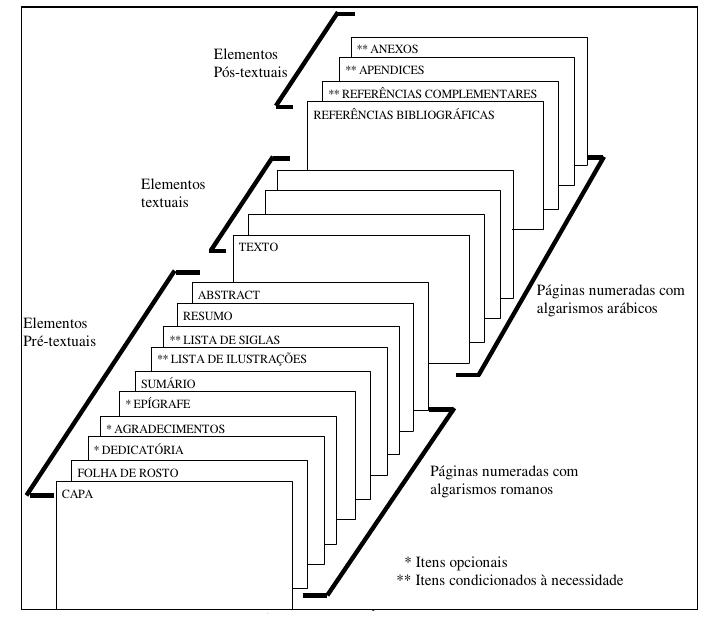
\includegraphics[width=160mm]{images/imagem2.jpeg}
  \end{center}
\end{figure}

\begin{itemize}
  \leading{5mm}
  \item [c)] \emph{Elementos Textuais} \\
  Aqui é o início do texto do relatório, a numeração é feita com algarismos
  arábicos, a partir do número 1.

  \begin{itemize}
    \item [-] Texto
  \end{itemize}

  \item [d)] \emph{Elementos Pós-Textuais} \\
  Os itens marcados com (*) são opcionais, isto é, só serão adicionados se o
  autor desejar.
  \item [-] Referências
  \item [-] Bibliografia recomendada(*)
  \item [-] Apêndices
  \item [-] Anexos
\end{itemize}

\section{Elementos Textuais}

\subsection{Introdução}
\subsection{Desenvolvimento}
\subsection{Conclusões e trabalhos futuros}
\section{Elementos Pós-Textuais}
\subsection{Referências bibliográficas}
\subsection{Bibliografia complementar}
\subsection{Apêndices}
\subsection{Anexos}
\section{Elementos de apoio ao texto}
\section{Editoração}
\subsection{Formatação de estilos}
\section{Conclusão}
\chapter{CAPITULO 3 - TESTE DE TÍTULO COM NOME GRANDE TESTE DE TÍTULO COM NOME
GRANDE TESTE DE TÍTULO COM NOME GRANDE}
\section{Teste de título com nome grande Teste de título com nome grande Teste
de com nome grande}
\subsection{Teste de título com nome grande Teste de título com nome grande
Teste de título com nome grande}
\section{Conclusão}
\chapter{CAPÍTULO 4}
\section{Formatando Tabelas}
\subsection{Sub-título aa}
\section{Sub-Título b}
\section{Conclusão}
\chapter{CONCLUSÕES}
\section{Considerações Finais}
\section{Trabalhos Futuros}

\begin{table}[ht]
\caption{Lemas mais usados por Cícero (cima pra baixo, esquerda pra direita)}
\begin{center}
\begin{tabular}{|c|c|c|c|c|c|}
\hline
dico & uerbum & quantus & oportet & lex & anima \\ \hline
possum & populus & suis & auctoritas & modius & liber \\ \hline
uideo & uita & ciuis & quaero & ars & exercitus \\ \hline
homo & animus & suo & facilis & arbitror & reliquus \\ \hline
facio & tuus & suus & prouincia & quin & praetor \\ \hline
causa & scribo & sententia & studium & genus & honor \\ \hline
habeo & multus & semper & loco & uirus & diligo \\ \hline
uolo & lego & nullus & intellego & plus & bene \\ \hline
iudex & consilium & ceterus & corpus & periculum & bellum \\ \hline
tantus & ius & saepe & dignitas & optimus & sentio \\ \hline
bonus & oratio & maior & pater & soleo & domus \\ \hline
ratio & inquam & uir & dolor & scriba & sapio \\ \hline
primus & dies & totus & scio & opus & rego \\ \hline
publica & gener & pars & do & dica & diu \\ \hline
maximus & uirtus & iudicium & ago & modus & imperium \\ \hline
tempus & pono & ueneo & necesse & proficiscor & plures \\ \hline
littera & itaque & pecunia & audio & mors & accipio \\ \hline
nunc & deus & minor & umquam & spes & praesertim \\ \hline
senatus & locus & debeo & fortuna & urbs & uno \\ \hline
uis & ciuitas & numquam & ullus & pario & malis \\ \hline
multa & consul & fors & omnino & duo & uoluntas \\ \hline
natura & satis & summo & orator & gratia & amicus \\ \hline
puto & nomen & animo & salus & memoria & moueo \\ \hline
magnus & publico & potis & utor & credo & mens \\ \hline
alter & solus & fero & uoluptas & populor & postea \\ \hline
\end{tabular}
\end{center}
\end{table}

\sigla{DDS}{Descrição da Sigla}
\sigla{DDS}{Descrição da Sigla}
\sigla{DDS}{Descrição da Sigla}
\sigla{DDS}{jkjk}

\end{document}